\documentclass[tikz,border=5pt]{standalone}
\usepackage{luatexja}
\usepackage[hiragino-pron]{luatexja-preset}
\usepackage{amsmath,amssymb}
\usepackage{pgfplots}
\pgfplotsset{compat=1.18}
\usetikzlibrary{arrows.meta,calc,decorations.markings,patterns,positioning}

% Common styles
\tikzset{
  axis/.style={-{Stealth[length=6pt]}, thick},
  curve/.style={thick, red},
  dashed curve/.style={thick, dashed, blue},
  dot/.style={circle, fill, inner sep=1.5pt},
  open dot/.style={circle, draw, fill=white, inner sep=1.5pt},
}

\begin{document}
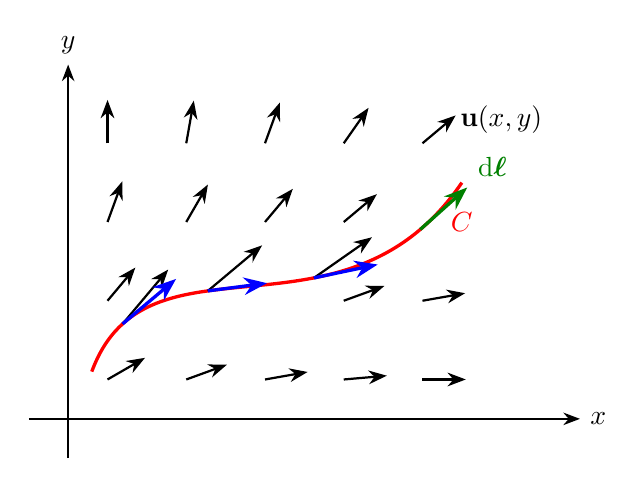
\begin{tikzpicture}[>=Stealth, thick]

  % Axes
  \draw[axis] (-0.5,0) -- (6.5,0) node[right] {$x$};
  \draw[axis] (0,-0.5) -- (0,4.5) node[above] {$y$};

  % Background vector field (black arrows, direction rotates from right to up)
  \foreach \x/\y/\ang in {
    0.5/0.5/30, 1.5/0.5/20, 2.5/0.5/10, 3.5/0.5/5, 4.5/0.5/0,
    0.5/1.5/50, 3.5/1.5/20, 4.5/1.5/10,
    0.5/2.5/70, 1.5/2.5/60, 2.5/2.5/50, 3.5/2.5/40,
    0.5/3.5/90, 1.5/3.5/80, 2.5/3.5/70, 3.5/3.5/55, 4.5/3.5/40
  }{
    \draw[->, thick] (\x,\y) -- ++(\ang:0.55);
  }

  % Curve C (red), extract pairs of nearby points for tangent directions
  \draw[very thick, red]
    (0.3,0.6) .. controls (1.0,2.5) and (3.5,0.8) ..
    coordinate[pos=0.14] (A) coordinate[pos=0.16] (A')
    coordinate[pos=0.39] (B) coordinate[pos=0.41] (B')
    coordinate[pos=0.64] (C) coordinate[pos=0.66] (C')
    coordinate[pos=0.89] (D) coordinate[pos=0.91] (D')
    (5,3.0);
  \node[red] at (5.0,2.5) {$C$};

  % At each point: black arrow = vector field u, blue arrow = tangent component of u
  % field angles at A, B, C (steeper than tangent to show projection)
  \foreach \P/\Q/\fang in {A/A'/50, B/B'/40, C/C'/35} {
    % Compute tangent angle
    \pgfmathanglebetweenpoints{\pgfpointanchor{\P}{center}}{\pgfpointanchor{\Q}{center}}
    \edef\tang{\pgfmathresult}
    % Black arrow: vector field u at this point
    \draw[->, thick] (\P) -- ++(\fang:0.9);
    % Blue arrow: tangent projection = |u| cos(field - tangent) along tangent
    \pgfmathsetmacro{\proj}{0.9*cos(\fang-\tang)}
    \draw[->, blue, very thick] (\P) -- ++(\tang:\proj);
  }

  % Green arrow: dℓ at point D (tangent)
  \pgfmathanglebetweenpoints{\pgfpointanchor{D}{center}}{\pgfpointanchor{D'}{center}}
  \edef\tangD{\pgfmathresult}
  \draw[->, green!50!black, very thick] (D) -- ++(\tangD:0.8)
    node[above right] {$\mathrm{d}\boldsymbol{\ell}$};

  % u(x,y) label
  \node at (5.5,3.8) {$\mathbf{u}(x,y)$};

\end{tikzpicture}
\end{document}
